\chapter{Engineering}

\section{Overview}

Next to project management and product assurance, engineering is the third branch of a space project. And it is the most essential one, as it produces the actual product or artefact, which is to achieve/deliver the mission objectives. In fact, project management and product assurance are merely functions (but very important one) that support and guide the engineering process. In this chapter we have a detailed look on the various aspects of engineering a space product.

\section{Engineering Disciplines}

In order to implement the system engineering process, a number of system engineering disciplines are involved. They are described in the following sections.

\subsection{System Engineering}
\label{sec:System Engineering}

\begin{tabular}{l}
\textit{ECSS-E-ST-10 "System engineering general requirements" \cite{ECSS-E-ST-10}}
\end{tabular}

System engineering is a multidisciplinary activity that transforms all technical requirements of the system into a system solution. A system is defined as an integrated set of elements to accomplish a defined objective. These elements include hardware, software, firmware, human resources, information, techniques, facilities services, and other support elements.

The concept of "system" is used here in a wide sense. The highest level, often called "mission level" or "space system", consists usually of one (or more) space segment(s), a ground segment, a launch segment, and a user segment. Elements of system decomposition are also considered a system. Hence, a system can be any element at any level of decomposition as defined by the function tree or the product tree. The scope of an element can include hardware, software, procedures, facilities and services.

The overall objective of system engineering is to obtain a product that satisfies the customer technical requirements within defined budget and time constraints. It includes the activities of definition of requirements, analysis, design and development, and verification. This is applied on all levels of the system. 

The governing document for all the system engineering activities is the \textbf{system engineering plan} (Section \ref{sec:System Engineering Plan}. The SEP gets input from other disciplines, including project management, product assurance, other engineering disciplines, production, operations and logistics. The SEP is continuously updated through the course of the project.

The traditional approach for conducting space system engineering is the waterfall approach, at which the following processes are carried out subsequently (corresponding to the project phases): definition of requirements, system design and production, and system verification.

\subsubsection{Requirements Engineering}

Requirements define the required technical performance of the system. Requirements are established on all levels of the system, and usually are elaborated from top to bottom. For example, a single high level requirement may be split into a number of low level requirements. This is done recursively until requirements on the lowest level are defined. To visualize the requirements, a specification tree may be used. However, to keep the tree manageable, the equipment element level requirements (and below) are usually put on a separate tree.

It must be ensured that requirements are consistent on all levels, that is, that they not contradict one another. Each requirement must be have the characteristics of being: traceable, unique, single, verifiable, unambiguous.

For being \textbf{traceable}, it must be clear from where the requirement originates, e.g. from a higher level requirements, an imposed constraint, and so on. For this, a requirement traceability matrix is used. For being \textbf{verifiable}, one or more methods must be identified for each requirement that will be used for its verification. \textbf{Unique} means that there must not be duplicated requirements, and \textbf{single} means that a requirement shall only cover one specific performance characteristic. \textbf{Unambiguous} means that requirements shall be written in a clear and precise way that leaves no room for interpretation.

There are several types of requirements, of which all or a subset may be applicable to the system element under consideration. ECSS-E-ST-10-06 \cite{ECSS-E-ST-10-06} provides details on the different requirements types and how to adequately define requirements. The list of requirements shall then be compiled in a \textbf{technical requirements specification} (Section \ref{sec:Technical Requirements Specification}). 

The source of requirements are manifold. For each project there are mission and project specific requirements. In addition, there is also a large number of generic requirements. Many requirements originate from mission analysis, which includes among others the analysis of the \textbf{space environment} (ECSS-E-ST-10-04 \cite{ECSS-E-ST-10-04} provides environmental models). Also non-technical factors, such as programmatic or product assurance constraints influence the system design. Generic requirements originate from applicable standards and expectations of common functionality and performance (ECSS-E-70-11 \cite{ECSS-E-ST-70-11} provides requirements on space segment operability).

Another important set of requirements are interface requirements. They are established with the objective to achieve functional and physical compatibility amongst all interrelated items in the product tree. ECSS-E-ST-10-24 \cite{ECSS-E-ST-10-24} provides a detailed list of reference interface data as a baseline for a \textbf{interface requirements document} (which itself is part of the technical requirements specification). 

Requirements are collected in a requirements database and by all means should not be changed after the completion of the requirements definition phase. A late change of requirement (e.g. during production phase) will likely incur high costs.

\subsubsection{Analysis}

Analysis is performed for decomposition of requirements and functional requirements analysis, resolving requirement conflicts, and estimating system performance. It is used to support the requirements engineering and the design process.

As an input to requirement engineering, the system engineering team shall perform an analysis of the \textbf{mission statement document} (Section \ref{sec:Mission Statement Document}) to produce the \textbf{mission description document} (Section \ref{sec:Mission Description Document}). For the case where several mission scenarios shall be compared and traded-off with each other, separate mission description documents, together with system engineering and project management plans are created. The winning concept is then chosen and document in a \textbf{system concept report} (Section \ref{sec:System Concept Report}).

Next, the functional architecture shall be established in form of a \textbf{function tree}. The function tree shall satisfies the customer requirements in terms of functionality, that is, the mission objective shall be composed into functional requirements.

In support of the design process, the system engineering team performs physical analysis to produce the \textbf{physical architecture} and the \textbf{product tree} (see Figure \ref{fig:Example of Product Tree}) of the system. Analysis is further used to justify the selected physical architecture. This includes a very wide range of analyses, such as thermal analysis, attitude and orbit analysis, data link analyses, etc. Performance analysis is to be performed on various levels of the system architecture, including end-to-end evaluation of the complete system. Analysis may also be performed to identify the impact of system imposed constraints to the cost and schedule of the project. 

All analyses are to be documented in analysis reports (Section \ref{sec:Analysis Report}).

\subsubsection{Design}

The design and development process produces a physical architecture of the complete system in terms of functionality and all the hardware and software characteristics.

The two main artifacts produced by the system engineering team are the \textbf{design definition file} (Section \ref{sec:Design Definition File}) and the \textbf{design justification file} (Section \ref{sec:Design Justification File}). Both are data repositories that hold references to all the information produced during the system design process. 

The design definition file (DDF) covers the technical definition of the system or product that complies with its technical requirements specification. The main aspects of the DDF are:

\begin{itemize}
\item Functional description (functional architecture, function tree, function chains)
\item Physical description (physical architecture, product and specification tree, element and interface description, technical budgets, margins, deviations)
\item Design constraints (constraints related to production, logistics, operation, maintainability)
\end{itemize}

The interfaces of the system are maintained in a dedicated \textbf{interface control document} for each interface (Section \ref{sec:Interface Control Document}) 

The design justification file (DJF) on the other hand is used to represent the rationale for the selected design solution, and to demonstrate that the design meets the requirements. The main aspects of the DJF are:

\begin{itemize}
\item Justification of functional architecture
\item Justification of physical architecture
\item Verification activities and reports
\item Justification of system budgets and margins
\item Justification of constraints imposed by system design
\end{itemize}

During the design process the system engineering team is working on the establishment and maintenance of the design definition file and the design justification file, and produces a \textbf{product user manual} (Section \ref{sec:Product User Manual}) that provides information on the design, operations, and data of the system that is required by the user to handle, install, operate, maintain, and dispose the product during its life time. If the system is a space segment, the product user manual (PUM) to produce is called \textbf{space segment user manual} (SSUM) (Section \ref{sec:Space Segment User Manual}).

Other supporting documents are the technical budget document and the coordinate system document. The \textbf{technical budget document} (Section \ref{sec:Technical Budget Document}) contains the various technical budgets of the system and may also record the evolution of the budgets over time. The \textbf{coordinate system document} (Section \ref{sec:Coordinate System Document}) is used to establish the reference coordinate systems to be used throughout the project.

\subsubsection{Verification}
\label{sec:Verification}

\begin{tabular}{l}
\textit{ECSS-E-ST-10-02 "Verification" \cite{ECSS-E-ST-10-02}} \\
\textit{ECSS-E-HB-10-02 "Verification guidelines" \cite{ECSS-E-HB-10-02}}
\end{tabular}

Verification has the objective to demonstrate that the deliverable products conform to the specified requirements. The verification process activities consist of planning, execution, and reporting and close-out. 

The verification planning is documented in the \textbf{verification plan} (Section \ref{sec:Verification Plan}) and covers the verification approach,model philosophy, methods, levels, stages, and verification tools. 

The \textbf{verification approach} activity is started early in the project life cycle. It analyzes which, how, and when requirements shall be verified, taking into account constraints and other factors. For each requirement to be verified, the verification strategy shall be defined in terms of verification methods, level, and stages. This is summarized in the \textbf{verification control document} (Section \ref{sec:Verification Control Document}) also known as verification matrix, which is to be approved by the customer.

The \textbf{model philosophy} defines the physical models that are required to achieve confidence in the product verification. The philosophy to be chosen depends on several factors, such as risk level, heritage, programmatic constraints, and budget. There are two dominant philosophies: prototype and protoflight. In the first approach separate models for qualification and acceptance are produced, whereas in the protoflight approach one model undergoes both verification stages. Hence the protoflight approach is cheaper but more risky, and suitable for systems with flight heritage.

The usual approach for new developments is therefore the prototype philosophy. An example of such a prototype philosophy and the associated models is shown in Figure \ref{fig:Example of Prototype Philosophy}.

\begin{figure}[h]
\centering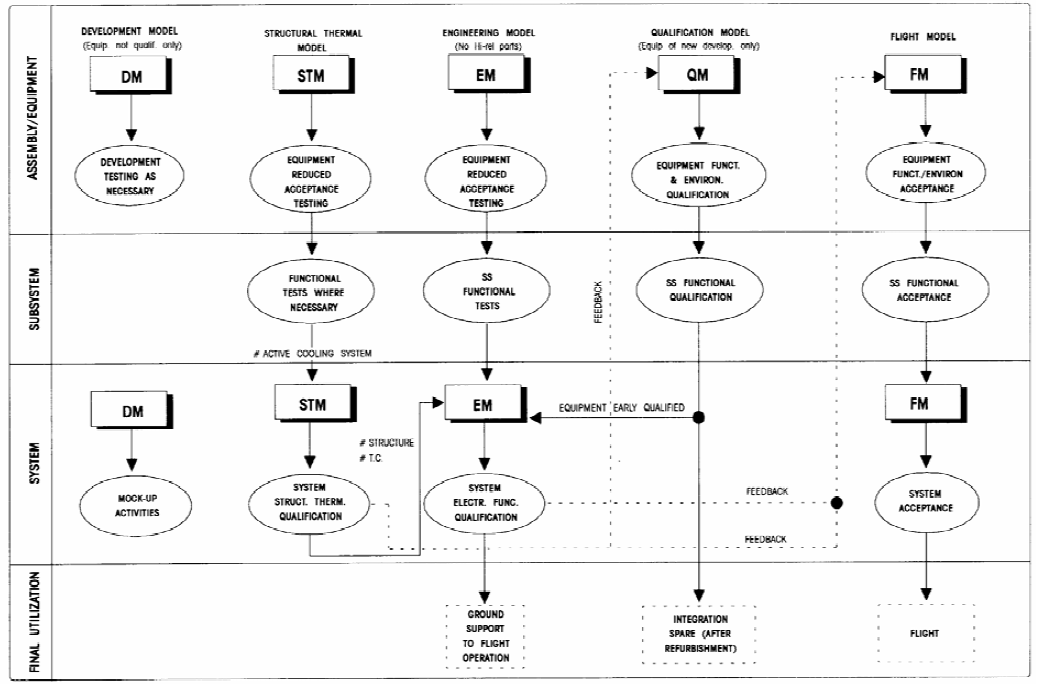
\includegraphics[scale=0.4]{fig/example_of_prototype_philosophy}
\caption{Example of Prototype Philosophy (ECSS)}
\label{fig:Example of Prototype Philosophy}
\end{figure}

Commonly defined models for verification programs are:

\begin{itemize}
\item \textbf{Development model} (DM): Used in general for new design or when substantial redesign is performed. Applicable to every type of product (e.g. electronic box, mechanisms, structural parts and thermal equipment) and can be subjected to functional and/or environmental testing. DM are sometimes also called bread board model.
\item \textbf{Structural model} (SM): Fully representative of the end product for structural aspects. Used for qualification of the structural design and for mathematical models correlation. Generally, the system structural model consists of a representative structure, with structural dummies of the flight equipment. It also includes representative mechanical parts of other subsystems (e.g. mechanisms and solar panels). The SM is also used for a final validation of test facilities, GSE, and related procedures.
\item \textbf{Thermal model} (ThM): Fully representative of the thermal properties of the end product. Used for the qualification of the thermal design and for the correlation of mathematical models. 
\item \textbf{Structural-thermal model} (STM): Combines the objectives of the SM and ThM.
\item \textbf{Suitcase model} (ScM): Intended to be used with the ground station for verifying correct telemetry (TM) reception, telecommand (TC) commanding. It is representative of the RF receiver and transmitter as well as the data handling part involved in the TM/TC protocol. 
\item \textbf{Electrical and functional model} (EFM): Functionally representative of the end products in both electrical and software terms. They are used for functional and interface tests and for failure mode investigations. Some part can be simulated by software; the rest is using commercial parts. Also known as Flatsat.
\item \textbf{Engineering model} (EM): Flight representative in form, fit and function, without high reliability parts and usually without full redundancy. The EM is used for functional qualification and failure survival demonstration. The EM is also used for final validation of test facilities and GSE and the related procedures.
\item \textbf{Qualification model} (QM): Fully reflects the end product design in all aspects. The QM is
used for complete functional and environmental qualification tests. 
\item \textbf{Flight model} (FM): The flight end product. It is subjected to formal functional and environmental acceptance testing. 
\item \textbf{Flight spare} (FS): The spare end product for flight. It is subjected to formal acceptance testing.
\end{itemize}

The \textbf{verification methods} available to the verification engineer are:

\begin{itemize}
\item Test
\item Analysis
\item Review of design
\item Inspection
\end{itemize}

The list is ordered by the magnitude of confidence that each verification methods gives, with tests being the most reliable verification methods. Hence, all (safety) critical functions shall be verified by test.

\textbf{Tests} shall be conducted under representative simulated environments. Tests objectives shall be documented via a \textbf{test specification} (Section \ref{sec:Test Specification}), the test conduction via a \textbf{test procedure} (Section \ref{sec:Test Procedure}) and the test results via \textbf{test report} (Section \ref{sec:Test Report}). The overall test program encompassing all tests shall be defined in the \textbf{assembly, integration, and test plan} (Section \ref{sec:Assembly, Integration, and Test Plan}).

\textbf{Analyses} use either theoretical or empirical techniques, such as statistical analysis or computational simulation. Analysis also covers verification by similarity. Analyses are document in the \textbf{analysis report} (Section \ref{sec:Analysis Report}).

\textbf{Review of design} uses records or evidence (such as technical drawings) that show unambiguously that a requirement is met. Reviews of design are document in the \textbf{review of design report} (Section \ref{sec:Review of Design Report}).

\textbf{Inspection} consists of visual determination of physical characteristics. Examples are visual inspection of products against workmanship errors or checking the conformance of source code against the defined \textbf{coding standards}. Inspections are document in the \textbf{inspection report} (Section \ref{sec:Inspection Report}).

In case that a verification encompasses more than one of the above methods, a \textbf{verification report} (Section \ref{sec:Verification Report}) is produced in addition to the other types of reports.

Verification shall be accomplished through selected \textbf{verification levels}. The verification process proceeds from lower level to higher level, i.e. the overall space system is verified last. Usual verification levels are:

\begin{itemize}
\item Space system (= mission)
\item Segment (e.g. ground segment, space segment)
\item Element (e.g. spacecraft platform)
\item Subsystem (e.g. AOCS)
\item Equipment (e.g. star tracker)
\end{itemize}

The verification process runs through several subsequent \textbf{verification stages}, which are:

\begin{itemize}
\item Qualification
\item Acceptance 
\item Pre-launch
\item In-orbit
\item Post-landing (if applicable)
\end{itemize}

In the \textbf{qualification stage} the verification shall demonstrate that the design, including margin, meets the applicable requirements. Therefore the product to be verified must be representative of the end product in terms of design, materials, tooling, and methods. To decide which item to be verified for the qualification test the general rule is that newly developed items must undergo full qualification, whereas items with heritage must undergo no or delta qualification, depending on their heritage.

In the \textbf{acceptance stage} the verification shall demonstrate that the product is free of workmanship errors and that it is ready for operation. Acceptance verification is carried out on the final product. 

In the \textbf{pre-launch stage} the verification shall demonstrate that the product is ready for launch and early operations.

In the \textbf{in-orbit stage} the verification shall ensure that no degradation occurred during launch and early operations. This stage also serves to confirm the space and ground segment inter-operability and operational aspects that cannot be verified before launch. Further, during this stage the spacecraft payload is calibrated and tuned for operation.

Typical \textbf{verification tools} are: 

\begin{itemize}
\item Ground support equipment (GSE)
\item Software validation facility (SVF)
\item Simulators
\item Software tools for analyses
\item Integration and test facilities
\end{itemize}

\subsubsection{Testing}

\begin{tabular}{l}
\textit{ECSS-E-ST-10-03 "Testing" \cite{ECSS-E-ST-10-03}}
\end{tabular}

Although testing is part of the verification program, it is of such importance to the system development that it is elaborated in more detail in this section. On the other hand, the discussion here is focused on testing of system elements from equipment up to segment level but not about testing of the overall system (e.g. end-to-end test or system validation test). To be more exact, this section is concerned with testing of qualification and flight (including protoflight) models.

Testing is conducted in the qualification, acceptance, and pre-launch stages of the verification process, and normally applied subsequently from lower level to higher level system elements. That means that in the qualification stage, qualification testing is carried out with individual equipment, which is then assembled and tested on subsystem level, and so on. Only when all testing related to the qualification stage has been completed one moves to the testing related to the acceptance stage.

Different testing requirements are applied for space segment equipment (e.g. processing modules, actuators, sensors) and space segment elements (the assembled spacecraft model). 

The \textbf{test planning} comprises of the establishment of the test program and the test reviews. The test program is decomposed into \textbf{test blocks} covering one specific test aspect and may contain one or more individual tests. Each test block is accompanied by \textbf{test reviews}, namely a \textbf{test readiness review} (TRR) to verify before the start of the test activity that all conditions allow to proceed with the test, and a \textbf{post test review} (PTR) to formally declare the test completed. 

The \textbf{test documentation} comprises of the \textbf{assembly, integration and test plan}, the individual \textbf{test specifications}, \textbf{test procedures}, \textbf{test reports}, and all the test data. Tests that are not passed are subject to nonconformance control.
 
The \textbf{test conditions} shall be such as to resemble predicted environments plus margin. Further, aspects of product assurance, namely safety and cleanliness, shall be implemented. \textbf{Test tolerances} and \textbf{ test accuracies} shall be agreed with the customer. Recommended values for tolerances and accuracies are provided in ECSS-E-ST-10-03 \cite{ECSS-E-ST-10-03}.

\textbf{Testing of equipment} typically comprises the following test blocks (although not all tests are applicable to all equipment):

\begin{itemize}
\item General tests
	\begin{itemize}
	\item Functional and performance: full test of all functionality (including deployments), system modes, and performance.
	\item Humidity (if applicable): functional test under humidity.
	\item Life (if applicable): test life time of life limited equipment.
	\end{itemize}
\item Mechanical tests
	\begin{itemize}
	\item Physical properties: determine dimensions, interfaces, mass, CoG, and MoI of equipment in launch configuration.
	\item Acceleration
	\item Random vibration
	\item Acoustic
	\item Sinusoidal vibration
	\item Shock
	\end{itemize}
\item Structural integrity tests
	\begin{itemize}
	\item Leak (if applicable): to be conducted before and after pressure, thermal, and mechanical tests of pressurized or sealed equipment.
	\item Proof pressure and pressure cycling (if applicable)
	\end{itemize}
\item Thermal tests
	\begin{itemize}
	\item Thermal vacuum
	\end{itemize}
\item Electrical/RF tests
	\begin{itemize}
	\item Electromagnetic compatibility
	\item Magnetic
	\item ESD
	\end{itemize}
\item Mission specific tests
\end{itemize}

Equipment test details and test levels for qualification and acceptance can be found in ECSS-E-ST-10-03 \cite{ECSS-E-ST-10-03} as well. An example of a full test sequence for equipment is shown in Figure \ref{fig:Example of Equipment Test Sequence}. 

\begin{figure}[h]
\centering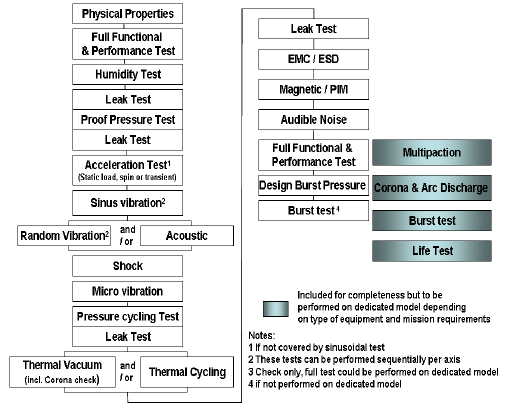
\includegraphics[scale=0.7]{fig/example_of_equipment_test_sequence}
\caption{Example of Equipment Test Sequence (ECSS)}
\label{fig:Example of Equipment Test Sequence}
\end{figure}

\textbf{Testing of spacecraft model} is to a large degree dependent on mission requirements and launcher profile. The following lists typical test blocks to be completed on spacecraft level, unless the launch provider requires different tests and/or test levels:

\begin{itemize}
\item General tests
	\begin{itemize}
	\item Functional (mechanical and electrical) and performance
	\item Mission: simulate nominal and contingency scenarios.
	\end{itemize}
\item Mechanical tests
	\begin{itemize}
	\item Physical properties: determine mass, CoG, and MoI of spacecraft in launch and orbit configuration.
	\item Modal survey
	\item Static load
	\item Spin
	\item Transient
	\item Acoustic
	\item Random vibration
	\item Sinusoidal vibration
	\item Shock
	\end{itemize}
\item Structural integrity tests
	\begin{itemize}
	\item Leak (if applicable)
	\item Proof pressure and pressure cycle (if applicable)
	\end{itemize}
\item Thermal tests
	\begin{itemize}
	\item Thermal vacuum
	\item Thermal balance
	\end{itemize}
\item Electrical/RF tests
	\begin{itemize}
	\item Electromagnetic compatibility
	\item Magnetic filed measurements
	\end{itemize}
\item Mission specific tests
\end{itemize}

Again, the test details and test levels for qualification and acceptance on spacecraft level can be found in ECSS-Q-ST-10-03 \cite{ECSS-E-ST-10-03}.

\textbf{Pre-launch testing} is very specific to the spacecraft and comprises at a minimum:

\begin{itemize}
\item Functional testing to verify that no damage or degradation has occurred during shipment and handling.
\item In case of assembly at launch site, the final configuration shall be retested.
\item Check of satellite health condition, such as battery status.
\end{itemize}

\subsection{Electrical Engineering}

\begin{tabular}{l}
\textit{ECSS-E-ST-20 "Electrical and electronic" \cite{ECSS-E-ST-20}}
\end{tabular}

The electrical engineering discipline covers all aspects of the electrical, electronic, electromagnetic, microwave and optical engineering processes design of space products. 

\subsubsection{General Requirements}

\textbf{Signal interfaces} design requirements:

\begin{itemize}
\item Ensure compatibility of characteristics of both sides.
\item Minimize number of interface types by using standard interfaces.
\item Critical signals shall include mechanisms (e.g. noise discrimination) to avoid spurious commanding.
\item Application of signals to an unpowered interface shall not cause damage.
\end{itemize}

\textbf{Command} design requirements:

\begin{itemize}
\item Executable commands shall be explicitly acknowledged in telemetry.
\item Critical commands shall consist of two separate commands for execution (e.g. arm and fire).
\item High priority commanding shall be independent from the main onboard processor and its software (this implies the high level command decoder, command generator, and their power supply to be entirely independent).
\item High priority commands shall only be issued under ground control.
\item Ground control shall be able to inhibit/deactivate any onboard commands, including critical commands.
\end{itemize}

\textbf{Telemetry} design requirements:

\begin{itemize}
\item Telemetry shall allow retracing of overall configuration as well as failure location at least to the level of all reconfigurable elements.
\item The operational status of each element shall be provided to determine validity of telemetry data from that element.
\item Main bus load currents and bus voltage shall be reported in telemetry.
\item Power-energy resources and source temperatures shall be reported in telemetry.
\end{itemize}

\textbf{Failure containment and redundancy} design requirements:

\begin{itemize}
\item A single failure shall not propagate outside a single reconfigurable element.
\item The spacecraft electrical system shall be single point failure free.
\item Redundancy functions shall be routed separately, e.g. via separate harness.
\item For hot-redundant essential units (e.g. receiver) latching protection shall not be used or shall have autonomous periodic reset.
\item Any protection latch without automatic reset capability shall be at least resettable by ground command.
\end{itemize}

\textbf{Data processing units} design requirements:

\begin{itemize}
\item Margins shall be defined at System Requirements Review for memory size, CPU load and throughput of onboard communications networks (minimum of 50\% for new developments).
\item In absence of specific requirements, the likelihood of reset or data corruption occurrence of main functions at equipment level shall be less or equal $10^{-4}$ per day for worst case conditions of environment.
\item Connectors that carry source power shall not expose contacts that could create short circuits (commonly female type connectors are used).
\item Connector shells shall be grounded, or if not possible, at least one contact of the connector shall be connected to the unit structure.
\item Erroneous connector mating shall be avoided by design.
\item Battery and solar array power shall be distributed on multiple contacts on both positive and return lines.
\end{itemize}

\subsubsection{Electrical Power}

Electrical power is used by all active spacecraft systems and equipment for their operation. Electrical power engineering includes power generation, energy storage,  conditioning, line protection and distribution. 

The power subsystem of a spacecraft shall be able to generate, store, condition, distribute and monitor the electrical power used by the spacecraft throughout all mission phases in the presence of all environments actually encountered.

Key aspect of power engineering are the power and energy budget. The \textbf{power budget} is based on analyzing the peak power demand versus the power available, whereas the \textbf{energy budget} is based on analyzing the average power versus energy available, taking into account spacecraft-sun distance, sun and eclipse durations, solar aspect angle, pointing, environmental effects, and possibly, failure scenarios.

The primary source for \textbf{energy generation} are solar arrays. Provision shall be made against potential failure propagation in case of short-circuit of a solar array section, namely by means of blocking diodes.

The primary mechanism for energy storage is \textbf{electrochemical energy storage}, namely batteries. The battery design shall include signal lines for monitoring of battery voltage and temperature, and the capability to charge or discharge the battery with ground support equipment before launch. Keep in mind that almost all battery technologies can be hazardous if not properly managed. The design of the battery shall therefore preclude the occurrence of over-temperature, excessive currents, overcharging and over-discharging.

The \textbf{power conditioning and control} has the task of providing a (regulated or unregulated) main bus power line from the solar array input in combination with the energy storage components (if available). No single point failure shall result in the loss of the power system in the sense that the minimum mission requirements cannot be met. Also, the following units shall be fully independent from any external control (such as on board computer): main bus voltage regulator, battery discharge control, and solar array controller (if available). In terms of performance, a fully regulated bus shall have a nominal ripple voltage below <TBD>\% of the nominal bus voltage. Bus under-voltage shall be prevented by implementing an autonomous (temporarily) disconnection circuit for non-essential loads. All such current limiting and auto switch-off circuits shall be monitored by telemetry.

In terms of \textbf{battery charge and discharge management}, the battery charger shall be able to ensure charging of batteries discharged down to zero volts. Also, the solar array power shall be enough to recharge the battery in any mission phase with all the essential loads connected or one worst case load connected (representing a failure), whichever is the more constraining.

The \textbf{power distribution and protection} has the task of routing the source power to the various loads. For this, the spacecraft structure shall be grounded, preferably at a star reference point. The switching of loads shall not generate a bus voltage transient exceeding <TBD>\% of the nominal bus voltage. The power lines shall be routed near ground and twisted. Harness shall not create stress at connector level, hence stress relief shall be implemented.

\subsubsection{Electromagnetic Compatibility}

The objective of electromagnetic compatibility (EMC) requirements is to ensure that the space system operates without performance degradation under self-induced and external electromagnetic environment. For cases where EMC is of concern during operation, ECSS-E-ST-20-07 \cite{} provides sufficient details.

\subsubsection{Radio Frequency Systems}

Radio frequency (RF) systems include transmitters, receivers, antennas and their  associated transmission lines (waveguides) including connectors. CubeSat RF system typically operate in the VHF band (30 to 300 MHz), UHF band (0.3 to 3 GHz) or S band (2 to 4 GHz). The transmitted or received signals can be narrowband or wideband, often with complex modulation. 

The RF engineering process takes into account:

\begin{itemize}
\item Antenna field of view and polarization
\item Link budget
\item Spatial and spectral resolution
\item Signal to noise ratio
\item Frequency plan
\end{itemize}

The RF design and development is concerned with transmitter power, receiver sensitivity, multipaction, spectral purity, VSWR, frequency stability, coupling between antennas, insulation, and EIRP.

\textbf{Antennas} are commonly in a stored configuration during launch, a deployment mechanism must be included, as discussed in Section \ref{ss:Mechanisms}. To avoid electrostatic discharge (ESD) all metallic parts of the radiating elements shall be connected to the equipment DC ground. The characteristics of antennas comprise coverage or beam shape, directivity, beam pointing, gain, input impedance mismatch factor, radiation patter, sense of polarization, side lobe level, noise temperature (for receive antennas), and variations of all those characteristics due to frequency, temperature, and ageing.

All RF equipment shall be able to stand the maximum specified \textbf{RF power} plus safety margin at maximum qualification temperature without degradation of components or radio signal. 

\subsection{Mechanical Engineering}
\label{ss:Mechanical Engineering}

The mechanical engineering discipline addresses all aspects of the mechanical design of space products. In particular it includes thermal control, structures including structural materials, mechanisms and pyrotechnics, and propulsion.

\subsubsection{Thermal}

\begin{tabular}{l}
\textit{ECSS-E-ST-31 "Thermal control general requirements" \cite{ECSS-E-ST-31}} \\
\textit{ECSS-E-HB-31-01 "Thermal design data handbook" \cite{ECSS-E-HB-31-01}} \\
\textit{ECSS-E-HB-31-03 "Thermal analysis handbook" \cite{ECSS-E-HB-31-01}}
\end{tabular}

The thermal control design goal is to keep each and every element of the spacecraft within its defined \textbf{temperature limits}, including acceptance and qualification margins, throughout the entire mission phase. Broadly, this can be achieved through passive and/or active thermal control. The latter introduces much complexity in terms of active control and feedback loops and additional equipment (e.g. heaters, sinks).

Thermal analysis focuses mostly on the worst case analysis of hot and cold cases. In the center of such analyses is the \textbf{thermal mathematical model} (TMM), which is a numerical representations of the item and its surrounding (models of which are defined in ECSS-E-ST-10-04 \cite{ECSS-E-ST-10-04}). The model is made up of concentrated thermal capacitance nodes that are coupled by a network of thermal conductors (radiative, conductive, and convective). Beforehand that however, the analysis process typically starts with the construction of a \textbf{geometrical mathematical model} (GMM) which is used to compute the radiative couplings and environmental heat exchanges, which drive the thermal behaviour of a spacecraft. The results of the radiative analysis computed with the GMM are then fed into the TMM which is used to compute temperatures and heat flows. 

\subsubsection{Structural}

\begin{tabular}{l}
\textit{ECSS-E-ST-32 "Structural general requirements" \cite{ECSS-E-ST-32}} \\
\textit{ECSS-E-HB-32-20 "Structural design data handbook" \cite{ECSS-E-HB-32-20}}
\end{tabular}

The structural engineering process produces a structural product with the objective to aim for simple load paths (simply geometry), maximizing use of conventional materials, simplifying interfaces, and providing easy integration. Structures have to withstand the applied loads caused by the natural and induced environments to which they are exposed to during their lifetime (including ground, launch, and operational environment conditions).

The mechanical environment shall be defined by thermal, static, and dynamic environment loads. The later two shall be defined in terms of constant acceleration, transient, sinusoidal, and random vibration, acoustic noise, and shock loads, each at their worst case levels (i.e. limit loads plus margin).

The characteristics of structures are strength, local yielding, buckling, stiffness, dynamic behavior, thermal behavior, tolerances and alignments, electrical conductivity, electromagnetic compatibility, and dimensional stability of the assembly. Key aspects of the structural design are inspectability, interchangeability, maintainability, dismountability, mass and inertia properties, and material selection (e.g. considering corrosion). The later is discussed in detail in ECSS-E-ST-32-08 \cite{ECSS-E-ST-32-08}. Structural design of spacecraft hardware shall include factors of safety. Those are discussed in detail in ECSS-E-ST-32-10 \cite{ECSS-E-ST-32-10}.

For the purpose of verification by analysis a \textbf{mathematical model} shall be developed. In most cases this is a \textbf{finite element model} as commonly used. ECSS-E-ST-32-03 \cite{ECSS-E-ST-32-03} provides requirements for its establishment. Such mathematical models shall always been validated by correlation with test results for specific needs. The analyses to be conducted with the model include static analysis (i.e. static loads), modal analysis (to confirm natural frequencies, see ECSS-E-ST-32-11 \cite{ECSS-E-ST-32-11}), and dynamic response analysis (due to excitations).

The structural engineer is also in charge of monitoring the mass and inertia properties via computation or preferable via measurement, where possible. 

\subsubsection{Mechanisms}
\label{ss:Mechanisms}

\begin{tabular}{l}
\textit{ECSS-E-ST-33-01 "Mechanisms" \cite{ECSS-E-ST-33-01}}
\end{tabular}

Mechanisms in space are often potential mission critical single point failures, and therefore particular attention must be placed upon the reliability and redundancy of such. Mechanisms shall be interchangeable and maintainable during storage and ground life. For the unlikely case of using explosive devices, they shall be designed in accordance with ECSS-E-ST-33-11 \cite{ECSS-E-ST-33-11}. 

\subsubsection{Propulsion}

Propulsion systems are currently in very early development stage for CubeSats and therefore this section only provides a brief overview on relevant standards.

ECSS-E-ST-35 \cite{ECSS-E-ST-35} provides the general requirements for propulsion propulsion systems. Associated \textbf{cleanliness} requirements are provided in ECSS-E-ST-35-06 \cite{ECSS-E-ST-35-06}.

Specific requirements for \textbf{liquid and electric propulsion} are provided in ECSS-E-ST-35-01 \cite{}. Further, ECSS-E-ST-35-10 \cite{} provides details on compatibility testing for liquid propulsion systems. 

Specific requirements for \textbf{solid propulsion} are provided in ECSS-E-ST-35-02 \cite{ECSS-E-ST-35-02}. 

\subsection{Software Engineering}

\begin{tabular}{l}
\textit{ECSS-E-ST-40 "Software" \cite{ECSS-E-ST-40} }
\end{tabular}

The software engineering discipline addresses the life cycle processes for software products (e.g. requirements definition, architectural design, development, operations and maintenance). In particular it addresses the different types of software: onboard (embedded), on ground, and software for qualification, testing and verification. 

Space software engineering is implemented in much the same way is space system engineering is. In fact, the term system as used in this section refers to the combination of hardware and software. When the software development is included in the overall CubeSat project, it will share the same project phases and reviews with it. An perhaps better alternative is to have the software development carried out as in individual project, with its on project phases and reviews. This is  a matter of choice. 

Either way, the following software project reviews are to be passed:

\begin{itemize}
\item \textbf{System requirement review}: Reach approval of the software requirements baseline.
\item \textbf{Preliminary design review}: Review compliance of technical specification with the requirements baseline, the software architecture, and the development plans.
\item \textbf{Critical design review}: Review the design definition file and the design justification file.
\item \textbf{Qualification review}: Review the validation against the requirements baseline.
\item \textbf{Acceptance review}: Review the completion of software delivery, installation, and acceptance.
\end{itemize}

In addition, a custom defined number of technical reviews may take place during the development. 

The following sections deal with the typical software development phases, independent of whether it is a standalone or integrated project. And although the phases and reviews suggest the use of a waterfall model, the \textbf{software development plan} (Section \ref{sec:Software Development Plan}, which is the central document describing the management and development approach, can implement any life cycle, such as an agile approach, through the means of the technical reviews.

An important activity that runs in parallel to all the ones discussed in the following is the \textbf{software verification process}. Broadly speaking it has the objective to ensure that the software engineering processes are implemented in accordance to a number of metrics and rules, as specified in ECSS-E-ST-40 \cite{ECSS-E-ST-40}. It is advisable to have someone appointed for the verification processes who is not involved in the development, in order to guarantee objectivity.

\subsubsection{Requirements and Architecture}

The system requirements allocated to the software are derived from the analysis of the specific intended use of the system (that is, the combination of software-hardware), and from results of safety and dependability analysis. It also includes the requirements on observability, which is the capability of being able to monitor the software behavior and to facility system integration and failure investigation. These requirements together constitute the \textbf{software requirements baseline} (RB).

When the requirements baseline has passed through the system requirement review, it is further elaborated into the \textbf{technical specification} (TS). the TS captures all requirements on lower level and cover therefore functional and performance specifications, operational, reliability, configuration, quality assurance, data definition, interface specification and so on.

The established technical specification is then transformed into a \textbf{software architecture}. The architecture describes the top-level structure of the software, identifies software components and their interrelation, and describes the static (packages, classes, units) and dynamic decomposition (threads, tasks, processes). Further, it shall described the software behavior.

\subsubsection{Design and Implementation}

The design and implementation process consists of the design of software items, the coding and testing, and the integration.

The design of software items shall be refined into lower levels containing \textbf{software units} that can then be coded, compiled, and tested. This includes the same aspects as outlined in the architectural design, namely the software units interfaces, relationships, and the description of static, dynamic, and behavioral aspects. The goal is to arrive at a detailed enough design and documentation (as captured in the \textbf{software design document}, Section \ref{sec:Software Design Document}) that allows \textbf{coding} without requiring further information.

The coding activity shall be accompanied with \textbf{software unit testing}. The goal of unit testing is to isolate each part of the program and show that the individual parts are correct. A unit test provides a strict, written contract that the piece of code must satisfy.

\subsubsection{Validation}

Whereas the unit testing focused on lower level testing, the validation process is conducted on higher level. Namely it has the objective of defining and carrying out tests for each of the requirements stated in the TS to validate against the technical specification, as well as for the requirements stated in the RB to validate against the requirements baseline.

\subsubsection{Delivery and Acceptance}

This process comprises the \textbf{transfer} of the software to and \textbf{installation on} the target platform. The \textbf{acceptance testing} is then carried out to demonstrate that the software runs as expected in the target environment.

The \textbf{software user manual} (Section \ref{sec:Software User Manual}) and the \textbf{software release document} (Section \ref{sec:Software Release Document}) are integral part of the software delivery.

\subsubsection{Operation}

For the case when the software is developed externally, the provision of \textbf{software operation support} during operations becomes essential. Software operation support shall provide means for re-coding and handling of problem reports (bugs) that are encountered by the user.

\subsubsection{Maintenance}

The maintenance activities are carried out when needed during the operation usage phase of the software. Maintenance falls in two categories: fixing or modification. Problem \textbf{fixing} is the response towards the problem reports that were filed by the user. For this, the problems are first analyzed to determine their type (e.g. corrective, preventive, adaptive), their scope (size, cost, time), and criticality (e.g. impact on performance, safety, security). The problem solution plan is then developed in accordance.

The \textbf{modification} of operational software is generally avoided unless necessary. A typical case for modification would be the migration from an old to a new target environment.

\subsection{Communications Engineering}

\begin{tabular}{l}
\textit{ECSS-E-ST-50 "Communications" \cite{ECSS-E-ST-50}}
\end{tabular}

Space communications engineering is concerned with the provision of end-to-end communication services between ground and space assets. The communication link is usually between space and ground, but may include spacecraft-to-spacecraft links (e.g. in constellations) or links between spacecraft and lander (including rovers). In any case, the typical stream of data is through the \textbf{uplink} from ground to space for the control of operations (\textbf{telecommands}), and through the \textbf{downlink} from space to ground for the transfer of \textbf{telemetry} (e.g. housekeeping and science data) or other service data. Because of this inequality of the nature of uplink and downlink, there are significant differences in the requirements of both.

For the control of operations via the uplink, the communication system has the objective to provide guaranteed delivery of commands in the order of transmission. Commands can be repeated, but not lost. By contrast, the objective of the communication system for the downlink is to transport as much data as possible. Some loss of data may be acceptable and even unavoidable, and the delivery order is generally not that important, provided that the data order can be reconstructed on ground.

The three distinct \textbf{space communication domains} are:

\begin{itemize}
\item \textbf{Space network}: The space network comprises all the nodes in the space segment. They can be on a single spacecraft (intra-spacecraft links) or distributed among several spacecraft (inter-spacecraft links). Typically, all space link related elements of the space network reside within the onboard communications subsystem, also referred to as telemetry, tracking and command (TT\&C) subsystem.
\item \textbf{Space link}: The space link is essentially a point-to-point wireless link (dominantly using radio frequencies, very seldom optical) between a ground station and a spacecraft. The space link is inherently unreliable and usually constrained in time. The medium through which the space link signal propagates can interfere and distort it and thereby introduce bit errors. In addition, the high relative velocity of most spacecraft creates a Doppler effect, which causes a varying shift in the radio signal frequency. Usually, separate frequencies are used for up- and downlink (full-duplex), such as UHF and VHF for many CubeSats. When only a single frequency is available, the up- and downlink can only be established one at a time (half-duplex).
\item \textbf{Ground network}: The ground network comprises of all ground-based equipment and the terrestrial links between them.
\end{itemize}

The two commonly found data containers are \textbf{packets} and \textbf{frames}. Packets encapsulate as their payload higher level data, which is part of some kind of service or higher level function. Frames on the other hand are containers for packets and may include a single, a fraction or several packets. The protocols and services associated with the communications system can be layered into five of the seven Open Systems Interconnection (OSI) model layers (omitting session and presentation layer):

\begin{itemize}
\item \textbf{Application layer}: Highest and most hardware-abstract layer of the OSI model. Application-layer functions correspond to the service functions provided by the specific software that implements it, such as file transfer or messaging services. Thus, this layer supports application and end-user processes. Communication partners are identified, quality of service is identified, user authentication and privacy are considered, and any constraints on data syntax are identified. Everything at this layer is application-specific.
\item \textbf{Transport layer}: Provides the function of transferring variable-length data sequences from a source to a destination host via one or more networks, while maintaining the quality of service functions. Some protocols on this layer are state- and connection-oriented. This means that the transport layer can keep track of the segments and retransmit those that fail. The transport layer also provides the acknowledgement of the successful data transmission and sends the next data if no errors occurred. 
\item \textbf{Network layer}: Provides the function of routing variable length higher-layer data encapsulated in packets from one node to another connected to the same network. It translates logical network address into physical machine address. A network is a medium to which many nodes can be connected, on which every node has an address and which permits nodes connected to it to transfer messages to other nodes connected to.
\item \textbf{Data link layer}: Provides node-to-node data transfer. It can be further divided into the \textbf{protocol sublayer} that specifies the layout of \textbf{frames} that transfer the data units provided by the higher layer, and the \textbf{synchronization and coding sublayer} that among other things adds capability to detect and possibly corrects errors that may occur in the physical layer.
\item \textbf{Physical layer}: Defines the electrical and physical specifications of the data connection (e.g. cable properties, radio frequency). This includes pin layout, voltage levels, signal timing, modulation, bit rate, and so on. 
\end{itemize}

In addition to the end-to-end transfer of commands and data, some other services are realized via the communication link as well, namely \textbf{time correlation} and \textbf{ranging}. Time correlation relates the local time at each communication end (e.g. the spacecraft onboard counter and the ground reception time) with each other to derive the absolute time of events and time stamps. Ranging is used to determine the distance between ground station and spacecraft to support orbit determination. Ranging has not been implemented yet for CubeSats. Instead, CubeSat projects rely on orbit parameters in the form of two line elements (TLEs) as generated via radar tracking by the North American Aerospace Defense Command (NORAD).

\subsection{Control Engineering}

\begin{tabular}{l}
\textit{ECSS-E-ST-60-10 "Control performance" \cite{ECSS-E-ST-60-10}} \\
\textit{ECSS-E-HB-60 "Control engineering handbook" \cite{ECSS-E-HB-60}} \\
\textit{ECSS-E-HB-60-10 "Control performance guidelines" \cite{ECSS-E-HB-60-10}}
\end{tabular}

The control engineering discipline addresses aspects of automatic control in space systems. Although control engineering is used in various elements and different levels of a space system,its dominant usage is for attitude (pointing) control. 

The purpose of control is to ensure that the output of the system does not deviate by more than a given amount from the target output (\textbf{performance error}). Mathematically speaking, the magnitude of physical quantity to be constrained shall remain below a defined maximum value with a certainty of greater or equal to a defined probability. That is, the difference between desired and actual value shall be kept within a defined limit (such error indices can be for example pointing errors or rate errors). This error is also influenced by the \textbf{knowledge error}, which is the difference between measured and actual value.

In order to determine whether or not the design of the control system meets the performance requirements there are various ways:

\begin{itemize}
\item \textbf{Experimental results}: This is usually not possible (at least on system level) until a late stage of the development. And even then, it may not be feasible, due to difficulties in simulating the target environment.
\item \textbf{Numerical simulations}: More practical than experimental results and therefore widely used. However, such simulations are often very time-consuming, for example Monte-Carlo simulations that comprises of a large number of simulations to cover many possible cases. Simulations are more useful for analyzing specific contributions to the total error rather than the total error for the entire system
\item \textbf{Compiled error budget}: This budget is used to estimate the total error given what is known about the individual contributing errors.
\end{itemize}

The fact that control engineering performance is strongly based on the theory of \textbf{probability} and \textbf{statistics} requires the engineer to have good understanding of these topics.

In addition to performance requirements, an essential property is \textbf{stability} and \textbf{robustness}. For linear systems, stability is an intrinsic performance property and does not depend on the type and level of the inputs. This does not hold for non-linear systems. Nonetheless, stability and robustness must be demonstrated over the whole uncertainty domain. This is commonly accomplished through gain and phase margins for single-input single-output (SISO) loops, or sensitivity functions for multi-input multi-output (MIMO) loops.


\subsection{Attitude and Orbit Control Engineering}

\begin{tabular}{l}
\textit{ECSS-E-ST-60-30 "Satellite attitude and orbit control system requirements" \cite{ECSS-E-ST-60-30}}
\end{tabular}

The following functions are typically covered by classical attitude and orbit control systems:

\begin{itemize}
\item Attitude estimation
\item Attitude guidance
\item Attitude control
\item Orbit control
\item Orbit estimation / Navigation
\item FDIR operations related to AOCS
\end{itemize}

Depending on the complexity and requirements of the specific CubeSat mission, attitude operations and orbit control may be implemented and carried out autonomously onboard, whereas orbit guidance is typically performed by ground segment. This standard provides requirements and performance definitions.

\subsection{Ground Systems Engineering}

\begin{tabular}{l}
\textit{ECSS-E-ST-70 "Ground systems and operations" \cite{ECSS-E-ST-70}}
\end{tabular}

Large part of the previous sections were only concerned with spacecraft system engineering. The engineering of the ground system however is conducted in a very similar pattern. Namely, the same project phases and reviews can be applied, and the process typically covers requirements analysis, design, development, and verification. 

An essential interface control document that governs the link between space and ground segment is the \textbf{space-to-ground interface control document} (SGICD, Section \ref{sec:Space-to-Ground Interface Control Document}). Another important aspect is logistics support that comprises the staffing of stations, the training, provision of spares and support equipment, and so on. Ground systems engineering is also tightly related to mission operations, which is presented in Chapter \ref{chap:Mission Operations}.

\begin{figure}[h]
\centering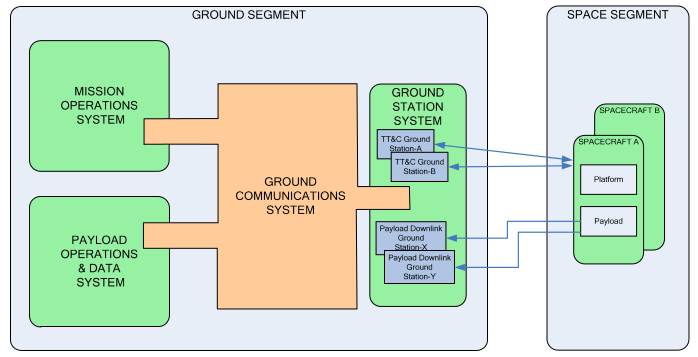
\includegraphics[scale=0.5]{fig/ground_segment_systems}
\caption{Ground Segment Systems (ECSS)}
\label{fig:Ground Segment Systems}
\end{figure}

The \textbf{ground segment} comprises all the \textbf{ground systems} that are used to support the preparation activities leading up to mission operations, the conduct of operations themselves and all post-operational activities. The ground segment as shown in Figure \ref{fig:Ground Segment Systems} typically consists of the following top-level systems:

\begin{itemize}
\item Mission operations system
\item Payload operations and data system
\item Ground station system
\item Ground communications system
\end{itemize}

\subsubsection{Mission Operations System}

The mission operations system typically supports the following:

\begin{itemize}
\item Mission analysis
\item Operations preparation
\item Simulation
\item Mission planning and scheduling
\item Monitoring and control
\item Flight dynamics
\item Onboard software maintenance
\item Data archiving
\item User services
\item Data product delivery
\item Performance analysis and reporting
\item Configuration management (space and ground segment, mission information)
\item System maintenance
\end{itemize}

\subsubsection{Payload Operations and Data System}

The payload operations and data system is used to exploit the mission products and typically supports:

\begin{itemize}
\item Payload operations analysis
\item Payload operations preparation
\item Simulation
\item Payload operations planning and scheduling
\item Payload operations control
\item Payload data processing
\item Payload data archiving
\item User services
\item Data product delivery
\item Performance analysis and reporting
\item Algorithm tuning and development, verification and validation
\item System maintenance
\end{itemize}

\subsubsection{Ground Station System}

The ground station system provides the physical link with the space segment. The following are supported, where applicable:

\begin{itemize}
\item Telemetry reception, storage and distribution
\item Telecommand transmission
\item Tracking, ranging, Doppler and meteorological data acquisition
\item Station monitoring and control
\item Time management
\item Network management and scheduling
\item Data distribution
\item System maintenance
\end{itemize}

\subsubsection{Ground Communications System}

The ground communications system provides the interconnections between systems, such as the connection between ground stations and mission control facilities. The following are supported, where applicable:

\begin{itemize}
\item Data distribution
\item Voice and video communication
\item System maintenance
\end{itemize}

\section{Model-Based System Engineering}

\begin{tabular}{l}
\textit{ECSS-E-TM-10-25 "Engineering design model data exchange (CDF)" \cite{ECSS-E-TM-10-25}} \\
\textit{ECSS-E-TM-10-23 "Space system data repository" \cite{ECSS-E-TM-10-23}} \\
\textit{CCSDS 311.0-M "Reference Architecture for Space Data Systems" \cite{CCSDS-311.0-M}} \\
\textit{"SysML Distilled: A Brief Guide to the Systems Modeling Language" \cite{delligatti2014sysml}}
\end{tabular}

To manage ever more complex systems and their interdependencies, there is a general trend in various engineering domains to move from a \textbf{document-centric} to a \textbf{model-centric} system engineering approach. Both approaches can equally be applied to the system engineering life cycle activities that were presented in the previous sections. The key difference between the two approaches, however, are the nature of the primary artifacts that they produce. 

With the \textbf{document-based} approach, systems engineers manually generate the documents related to system engineering, namely requirements specifications, interface definition documents, design definition documents, and so on. Document-based systems engineers produce these artifacts in the form of a disjoint set of text documents, spreadsheets, diagrams, and presentations (and configuration-manage them in a disjoint set of repositories). The problem is that the task of keeping all those documents in synch and up-to-date, is heavily time-consuming and error prone. Imagine for example just the profane activity of changing the name of an equipments unit; all documents making reference to it will have to be modified as well.

With the \textbf{model-based} system engineering (MBSE) approach, systems engineers perform the same life cycle activities and produce the same set of deliverables. But the deliverables are not the immediate outputs of the life cycle activities; they are not the primary artifacts. With the MBSE approach, the primary artifact of those activities is an integrated, coherent, and consistent system model, created by using a dedicated systems modeling tool. All other artifacts are secondary and automatically generated from the system model using that same modeling tool, which serves as the central repository for the design.

There are three things needed to conduct MBSE, namely:

\begin{itemize}
\item Modeling language
\item Modeling method
\item Modeling tool
\end{itemize}

To create a model, a \textbf{modeling language} is needed first. This is a semiformal language that defines the kinds of elements that can be put in the model, the relationships these elements can have with each other, and the set of notations that can be used to display them visually. The modeling language of choice that has found widespread acceptance is the \textbf{Systems Modeling Language (SysML)}.

While the language specifies the set of rules to determine if a given model is well formed or not, it does not prescribe anything about how to actually construct such a model. It is the chosen \textbf{modeling method} that dictates how and when models shall be created. At present there is no formally established method, but the one described in ECSS-E-TM-10-25 \cite{ECSS-E-TM-10-25} may serve as a good reference.

Not less important is the \textbf{modeling tool}. The tool must comply with the grammar of the modeling language. But different to simple drawing tools that only show diagrams that are drawn following the grammar of the modeling language, the modeling tool must also support the creation of the model itself, which serves as the underlying model for creating such views, and the integrated consistency updates. Although the prospects of MBSE are promising, such tools, in particular those in the open domain, are still not very mature. In addition, the semantics and reference models for use in space system engineering are yet to be formally established.

\clearpage
\section{Deliverables}
\label{sec:Engineering Deliverables}

\subsection{Documents per Review}

\begin{table}[h]
\centering
\begin{tabular}{l c c c c c c c c c}
\toprule
\textbf{Phase} & \textbf{0} & \textbf{A} & \multicolumn{2}{c}{\textbf{B}} & \textbf{C} & \multicolumn{2}{c}{\textbf{D}} & \multicolumn{2}{c}{\textbf{E}} \\
\textbf{Review} & \textbf{MDR} & \textbf{PRR} & \textbf{SRR} & \textbf{PDR} & \textbf{CDR} & \textbf{QR} & \textbf{AR} & \textbf{ORR} & \textbf{FRR} \\
\midrule
Mission description doc.    	& • & • &   &   &   &   &   &   &   \\
\hline
System - TS              	    &(•)&(•)& • &   &   &   &   &   &   \\
\hline
System - I/F TS          	    &   &(•)& • & • &   &   &   &   &   \\
\hline
System engineering plan		    & • & • & • & • & • & • & • &   &   \\
\hline
Verification plan 		        &   & • & • & • & • & • & • &   &   \\
\hline
AIT plan						&   &   &   & • & • & • & • &   &   \\
\hline
Orbital debris mitigation plan	& • & • & • & • & • & • & • & • & • \\
\hline
Coordinate system doc.       	&   & • & • & • & • & • &   &   &   \\
\hline
\hline
Design definition file       	&   & • & • & • & • & • & • &   &   \\
\hline
Function tree               	&   & • & • & • &   &   &   &   &   \\
\hline
Product tree	                &   & • & • & • &   &   &   &   &   \\
\hline
Specification tree           	&   &   & • & • &   &   &   &   &   \\
\hline
Technical budget            	&   & • & • & • & • & • & • &   &   \\
\hline
Element - TS                    &   &(•)& • &   &   &   &   &   &   \\
\hline
Subsystem - TS                  &   &   &(•)& • &   &   &   &   &   \\
\hline
Interface control doc.          &   &   & • & • & • & • & • & • & • \\
\hline
Product user manual  	        &   &   &   &   & • & • & • & • & • \\
\hline
\hline
Design justification file      	&   & • & • & • & • & • & • &   &   \\
\hline
Verification control doc.       &   &(•)&(•)&(•)& • & • & • & • & • \\
\bottomrule
\end{tabular}
\caption{System Engineering Documents required per Review}
\end{table}

(•) = preliminary

\subsection{Documents per Request}

\begin{itemize}
\item Test specification
\item Analysis report
\item Test procedure
\item Test report
\item Review of design report
\item Inspection report
\end{itemize}
